% ============
% = Concepts =
% ============
\clearpage
\section{Program Creation Concepts} % (fold)
\label{sec:program_creation_concepts}

Our first program is going to display some text to the Terminal. In this section you will be introduced to the programming artefacts and terminology you will need to use to create this program. This first step is important and will require you to have installed a C++ or Pascal compiler, see \cref{cha:building programs} \nameref{cha:building programs} for instructions.

A programming \textbf{artefact} is something that can be created and used within your code. In this chapter we will look at creating programs, and using a number of other artefacts. The following artefacts will be covered in this chapter:
\begin{itemize}
  \item \nameref{sub:program}: A program is a sequence of instructions that when compiled creates an executable file that a user can run.
  \item \nameref{sub:procedure}: A procedure is a named sequence of instructions that will get the computer to perform a task. When you want the task performed you can call the procedure.
  \item \nameref{sub:library}: The program can use code from other Libraries. These libraries contain reusable Procedures and Types. 
  \item \nameref{sub:type}: A type defines how data is interpreted by the program. The programming language will support a number of basic types by default, and libraries can add other types. 
\end{itemize}

In addition to these artefacts, you will need to understand some programming \textbf{terminology}. The following terms are discussed in this section:
\begin{itemize}
  \item \nameref{sub:statement}: An \textbf{instruction} within the program.
  \item \nameref{sub:expression}: A \textbf{value} used in a statement.
  \item \nameref{sub:identifier}: The \textbf{name} of an artefact.
  % \item Literal: A part of an \textbf{expression} where the value is entered directly into the code.
\end{itemize}

This section also introduces the following kinds of instructions. You can use these to get the computer to perform certain \textbf{actions} within your program.
\begin{itemize}
  \item \nameref{sub:procedure call}: The instruction to run a procedure.
\end{itemize}

We can then use these concepts, artefacts, and instructions to create a program that will write some text to the Terminal as shown in Figure \ref{fig:program-creation-helloworld}.

\begin{figure}[h]
   \centering
   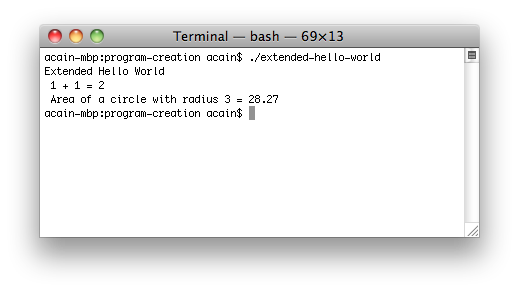
\includegraphics[width=0.8\textwidth]{./topics/program-creation/images/HelloWorld} 
   \caption[Hello World Terminal]{Hello World run from the Terminal}
   \label{fig:program-creation-helloworld}
\end{figure}

\clearpage
\subsection{Program} % (fold)
\label{sub:program}

A program contains the instructions the computer will follow when that program is executed. In your source code you can declare a program in which you code the steps you want followed when your program is executed. When you compile this code the compiler will create an executable file (a \emph{program}) that the user can run. Running the program will then get the computer to perform the steps you wrote in the code.

\begin{figure}[h]
   \centering
   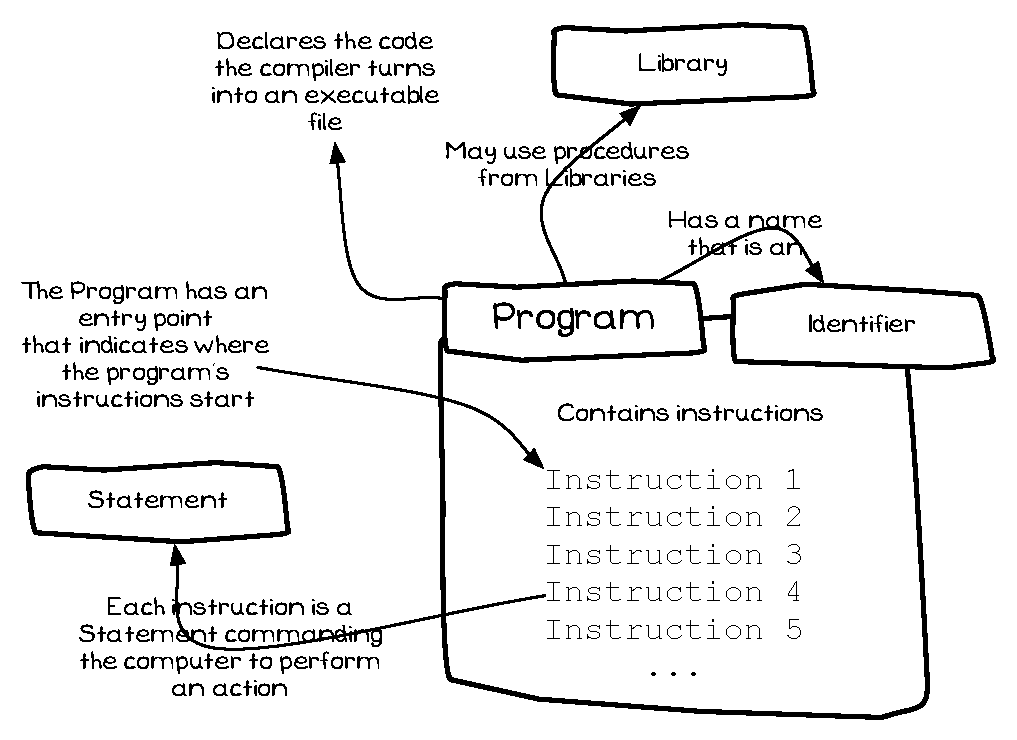
\includegraphics[width=\textwidth]{./topics/program-creation/diagrams/BasicProgramConcept} 
   \caption{A program contains instructions that command the computer to perform actions}
   \label{fig:program-creation-program}
\end{figure}


\mynote{
\begin{itemize}
  \item A program is an \textbf{artefact}, something you can create in your code.
  \item Figure \ref{fig:program-creation-program} shows the concepts related to programs.
  \item A program is a programming artefact used to define the steps to perform when the program is run.
  \item You use the compiler to convert the program's source code into an executable file.
  \item By declaring a program in your code you are telling the compiler to create a file the user can run.
  \item The program has an \textbf{entry point} that indicates where the program's instructions start.
  \item The name of the program determines the name of the executable file.
  \item Your program can use code from a \nameref{sub:library} or number of libraries.
  \item In programming terminology, an instruction is called a \nameref{sub:statement}.
\end{itemize}
}

% section program (end)
\clearpage
\subsection{Statement} % (fold)
\label{sub:statement}

A statement is an instruction for the computer to perform an action, a command telling it what to do. Each \nameref{sub:program} contains a list of statements (commands). When the program is run the computer follows these commands one at a time, in sequence, starting at the program's entry point and ending when it completes the program's last statement.

\begin{figure}[h]
   \centering
   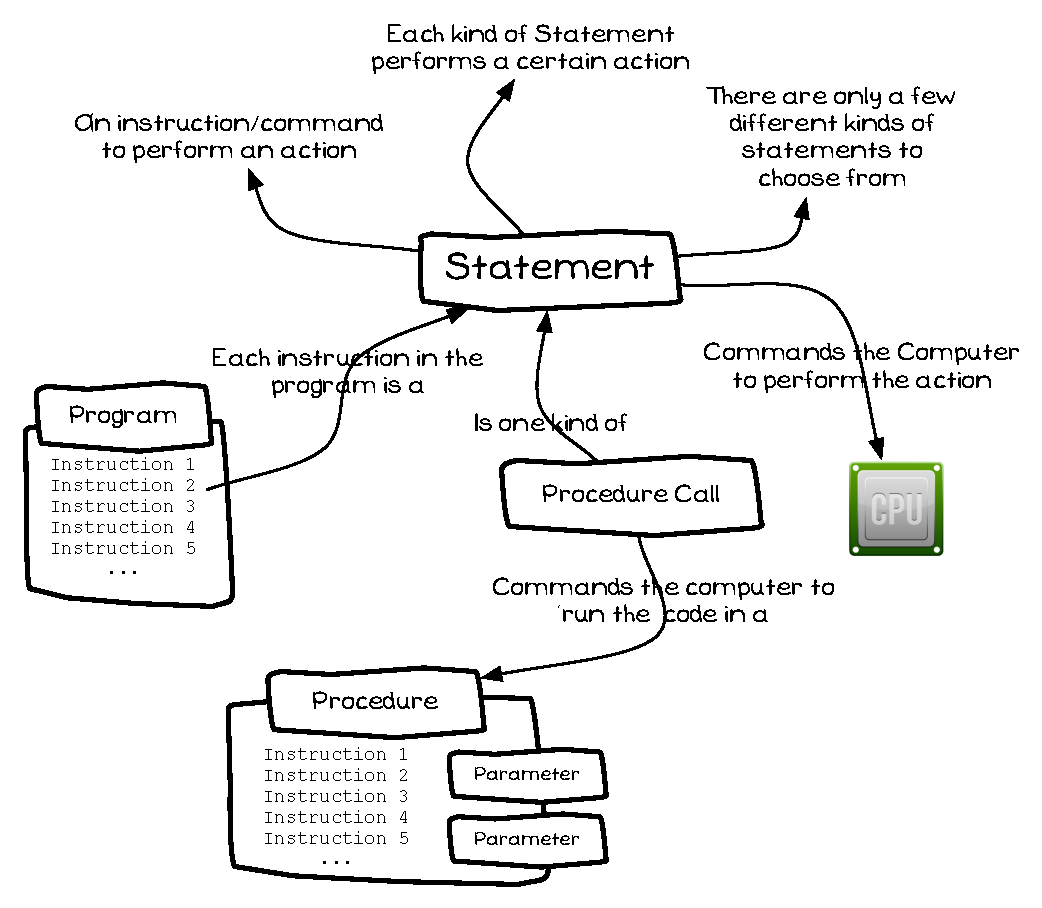
\includegraphics[width=\textwidth]{./topics/program-creation/diagrams/Statement} 
   \caption{A statement is a command for the computer to perform an action}
   \label{fig:program-creation-statement}
\end{figure}


\mynote{
\begin{itemize}
  \item A statement is a \textbf{term} used to describe the instructions in your code.
  \item Figure \ref{fig:program-creation-statement} shows the concepts related to statements.
  \item A statement is a \textbf{command}, an instruction to perform a task.
  \item A \nameref{sub:program} has a list of statements that are followed when it is executed.
  \item There are only a few different kinds of statement.
  \item A \nameref{sub:procedure call} is a kind of statement, it tells the computer to run the code in a \nameref{sub:procedure}.
  \item This style of programming is known as \textbf{Imperative} programming. Imperative means to give authoritative commands, and that is what we do in our programs. Our programs are lists of authoritative commands telling the computer to perform actions.
\end{itemize}
}

% section statement (end)
\clearpage
\subsection{Procedure Call} % (fold)
\label{sub:procedure call}

A procedure call is a kind of \nameref{sub:statement} that instructs the computer to run the code in a \nameref{sub:procedure}. If the procedure requires some data to work with, then this data is passed to the procedure as part of the procedure call. The procedure's name is used to identify the procedure to call.

\begin{figure}[h]
   \centering
   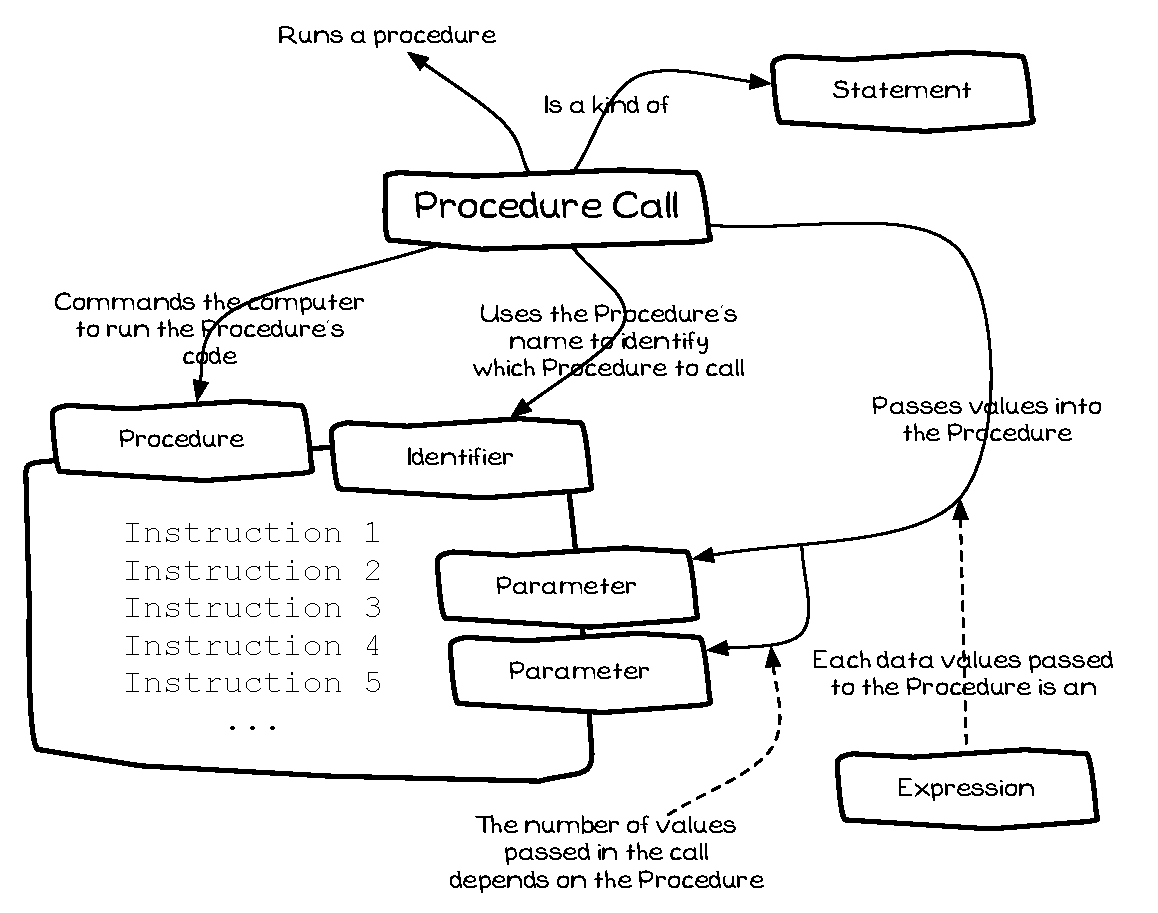
\includegraphics[width=\textwidth]{./topics/program-creation/diagrams/ProcedureCall} 
   \caption{A procedure calls runs a procedure, passing in values for the procedure to use}
   \label{fig:program-creation-procedure call}
\end{figure}


\mynote{
\begin{itemize}
  \item A procedure call is an \textbf{action}, you can call procedures in your code.
  \item Figure \ref{fig:program-creation-procedure call} shows the concepts related to the procedure call.
  \item A procedure call is an instruction to execute a procedure.
  \item You can code a procedure anywhere you can code a statement.
  \item The \nameref{sub:identifier} indicates the \nameref{sub:procedure} to call.
  \item Data values passed to the procedure are coded using \nameref{sub:expression}s.
  \item When the procedure's task is complete the program continues with the next \nameref{sub:statement}.
\end{itemize}
}

% section program (end)
\clearpage
\subsection{Procedure} % (fold)
\label{sub:procedure}

A Procedure is a part of a \nameref{sub:program} that performs a specific task. Each Procedure has a name that should reflect the task the procedure carries out. When a Procedure is called it gets control of the computer and instructs it to perform the steps needed to carry out the task the Procedure is responsible for. Often these tasks require data, so the Procedure may need to be passed data when it is called. When the procedure finishes its task control returns back to the code that called the Procedure.

\begin{figure}[h]
   \centering
   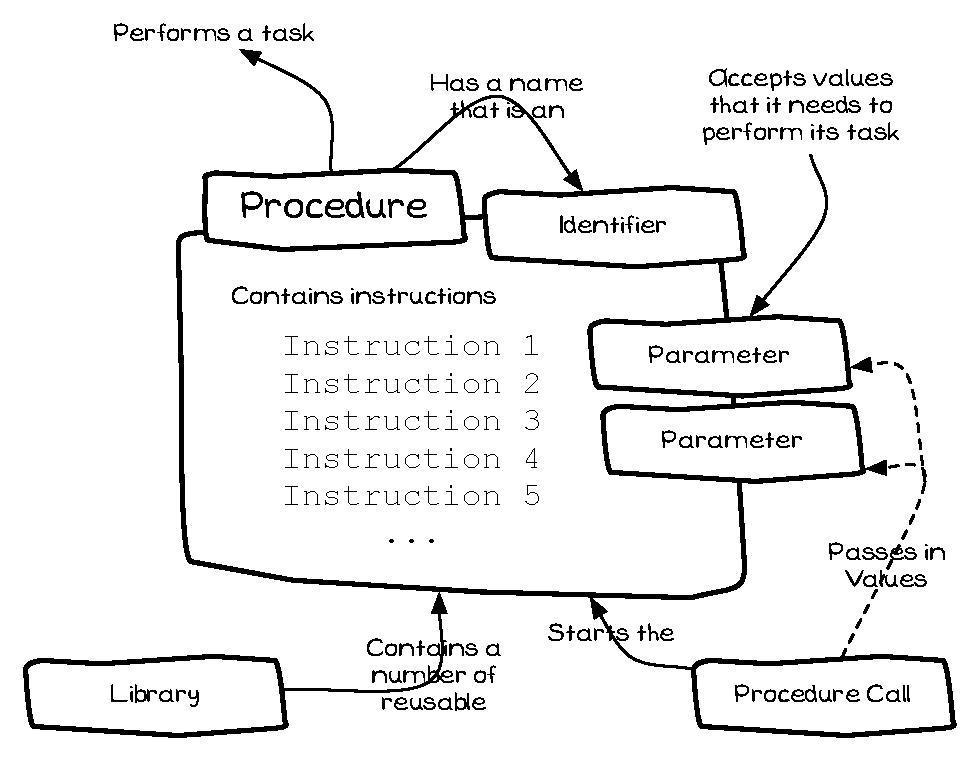
\includegraphics[width=\textwidth]{./topics/program-creation/diagrams/Procedure} 
   \caption[Procedure Concept Diagram]{A Procedure contains instructions to perform a task, and may need to be passed data in order to do this}
   \label{fig:program-creation-procedure}
\end{figure}


\mynote{
\begin{itemize}
  \item Figure \ref{fig:program-creation-procedure} shows the concepts related to Procedures.
  \item A Procedure is a programming artefact that can be called to perform a certain task.
  \item The name of a Procedure is an \nameref{sec:program-creation-identifier}.
  \item Each \nameref{sec:program-creation-library} will contain a number of Procedures to perform common tasks.
  \item The standard library will include procedures to write values to the console.
  \item The SwinGame libraries contain procedures that can draw images on the screen, play sounds, and perform other tasks needed to create small games.
  \item Procedures are also called \textbf{subroutines}, \textbf{sub programs}, \textbf{methods} or \textbf{sub procedures}.
\end{itemize}
}

% section program (end)
\clearpage
\subsection{Expression} % (fold)
\label{sub:expression}

An Expression is a value used in a \nameref{sec:program-creation-statement}. These values may be calculated or entered directly into the source code of the Program.

\begin{figure}[h]
   \centering
   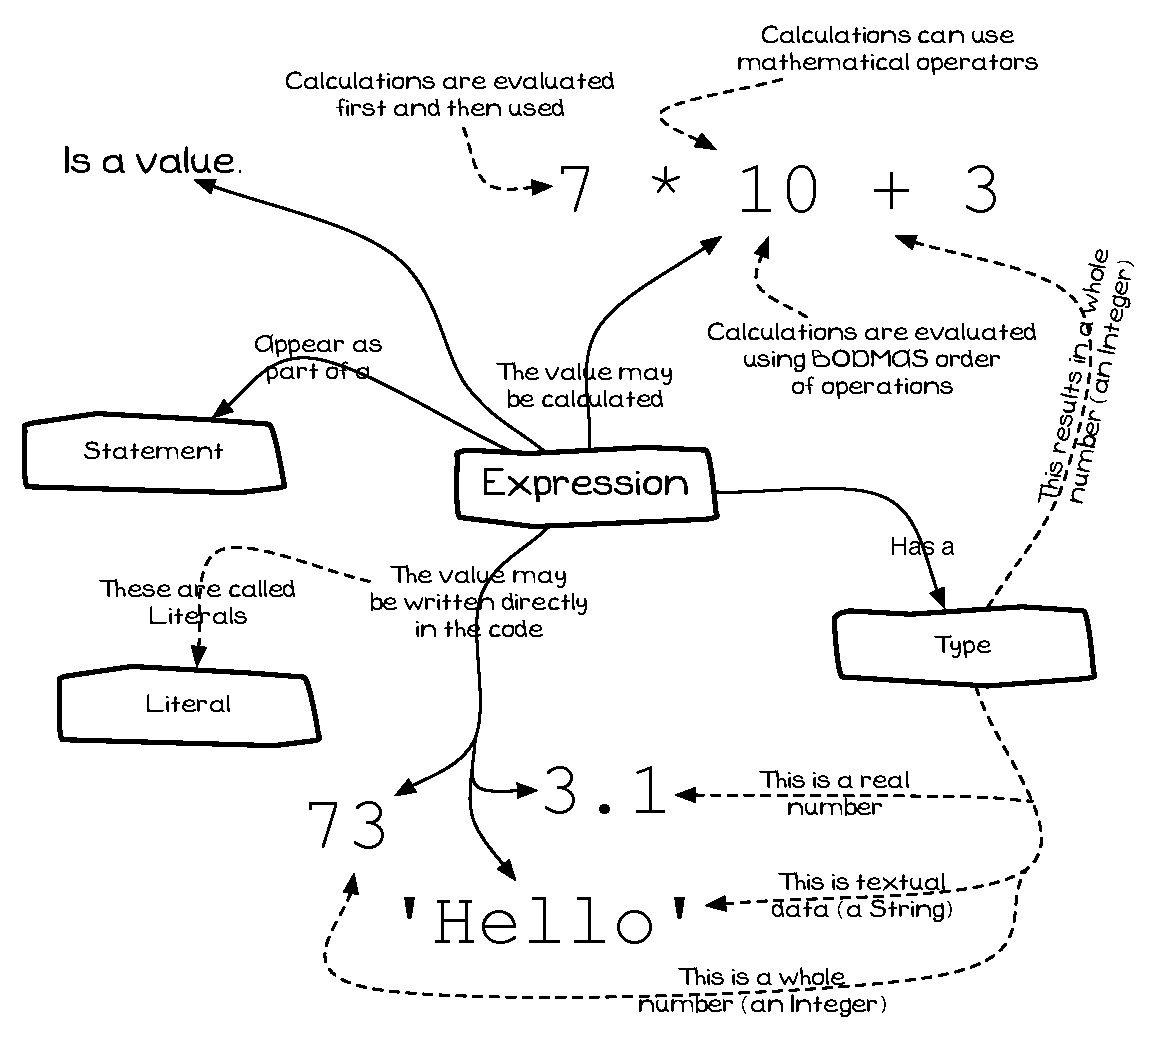
\includegraphics[width=\textwidth]{./topics/program-creation/diagrams/Expression} 
   \caption[Expression Concept Diagram]{An Expression provides a \textbf{value} to be used in a Statement.}
   \label{fig:program-creation-expression}
\end{figure}


\mynote{
\begin{itemize}
  \item The concepts related to Expressions are shown in Figure \ref{fig:program-creation-expression}.
  \item An Expression provides a \textbf{value} that is used in a Statement.
  \item The Expression's value may be calculated or entered directly into the code.
  \item Calculations can use mathematical operators: + for addition, - for subtraction, * for multiplication, $/$ for division, and parenthesis ( ) for grouping.
  \item Expressions are evaluated using the BODMAS order of operations.
  \item Values entered directly within an Expression are \textbf{Literal} values.
\end{itemize}
}

% section program (end)
\clearpage
\subsection{Literal} % (fold)
\label{sec:program-creation-literal}

A Literal is a whole, or part of, an \nameref{sub:expression} where the value is entered directly into the code.

\begin{figure}[h]
   \centering
   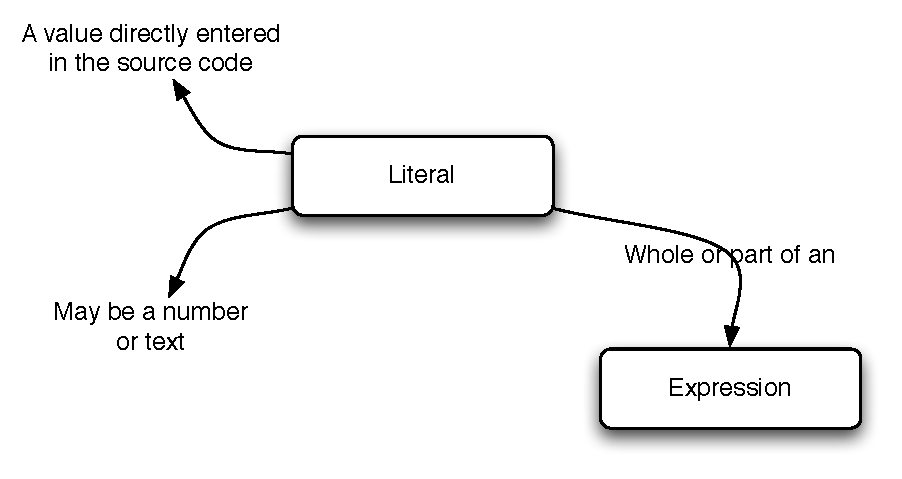
\includegraphics[width=0.8\textwidth]{./topics/program-creation/diagrams/Literal} 
   \caption[Literal Concept Diagram]{Concepts related to Literals.}
   \label{fig:program-creation-literal}
\end{figure}


\mynote{
\begin{itemize}
  \item Figure \ref{fig:program-creation-literal} shows the concepts relate to Literals.
  \item A Literal is a value entered directly into the program's source code.
  \item The value of a Literal can be a number or text.
  \item A Literal can be part or all of an \nameref{sub:expression}.
  \item These values are \emph{hard coded} into the program.
\end{itemize}
}

% section program (end)
\clearpage
\subsection{Type} % (fold)
\label{sub:type}

All values within a program will have a type. The type indicates how the data stored in the computers memory is interpreted by the program. There are three basic data types available in a programming language.

\begin{itemize}
    \item \textbf{Textual} data such as `\emph{Fred}', `\emph{Hello World}', `\emph{23}', and `\emph{This is text!}'.
    \item \textbf{Whole numbers} such as \emph{1}, \emph{0}, \emph{-5}, and \emph{37}.
    \item \textbf{Real numbers} such as \emph{0.5}, \emph{-126.0}, \emph{3.141516}, and \emph{23.981}.
\end{itemize}

\begin{figure}[h]
   \centering
   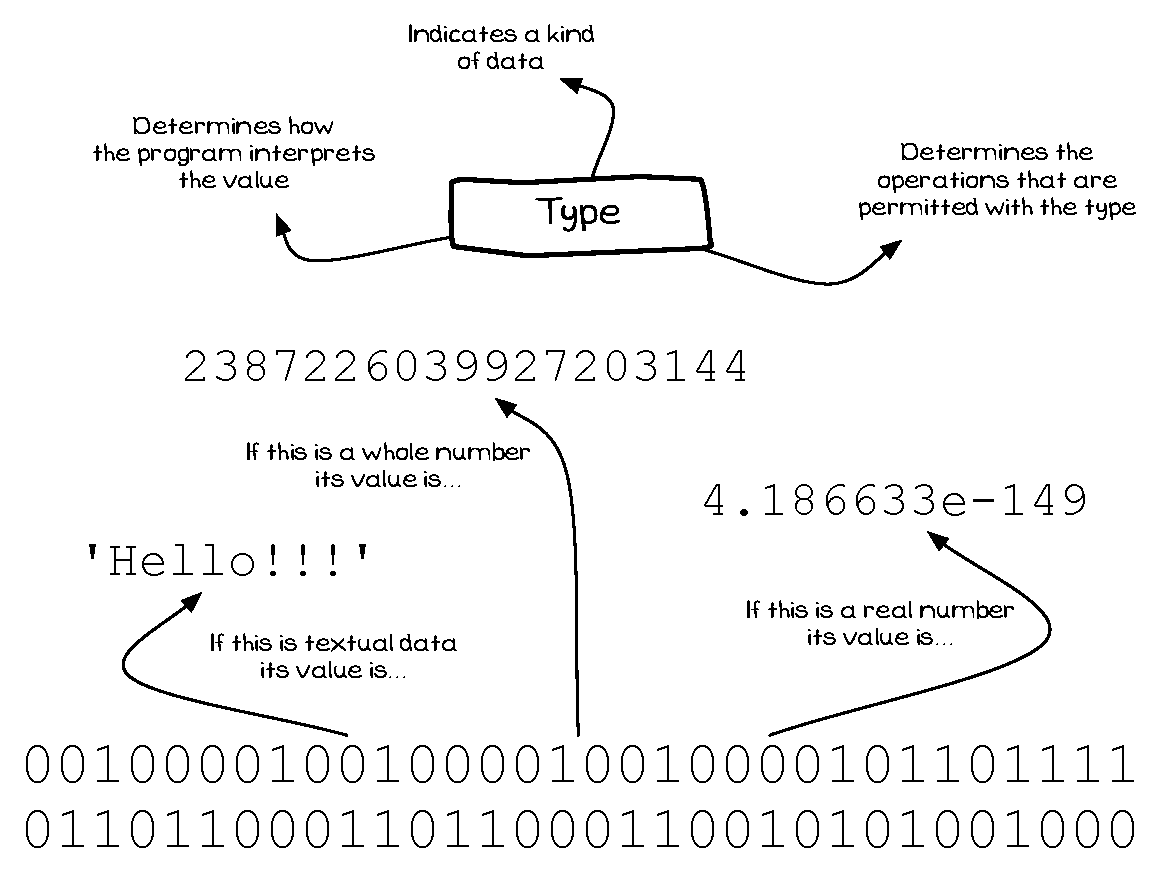
\includegraphics[width=0.95\textwidth]{./topics/program-creation/diagrams/Type} 
   \caption{Types defines how values are interpreted, and the operations that can be performed on the data}
   \label{fig:program-creation-type}
\end{figure}

\mynote{
\begin{itemize}
  \item A type is an \textbf{artefact}, there will be a number of existing types that you can use, and later you will see how to create your own types.
  \item The concepts related to expressions are shown in Figure \ref{fig:program-creation-type}.
  \item A type is a programming artefact that indicates a kind of data.
  \item The type determines the basic actions that can be performed on the value.
  \item The type determines the amount of memory needed to store a value of that kind.
  \item Whole numbers are usually called \textbf{Integers}.
  \item Real numbers are usually represented as \textbf{Floating Point} values. These values have a limited precision, supporting only a certain number of digits of precision.
  \item Textual values can contain numbers. In these cases the number are just textual representations of the values. For example, the text `\emph{23}' is the character `\emph{2}' followed by the character `\emph{3}', it is not the number \emph{23}.
  \item You can perform mathematic operations on numeric data, but not on textual data.
\end{itemize}
}

% section program (end)
\clearpage
\subsection{Identifier} % (fold)
\label{sub:identifier}

An Identifier is the technical term for the words that \emph{identify} something for the compiler. These can be the \textbf{name} of a programming artefact such as a Program, Library, or Procedure, or the words that have special means for the compiler. You will use Identifiers to name the artefact you create, and to select the appropriate artefact when it is used.

\begin{figure}[h]
   \centering
   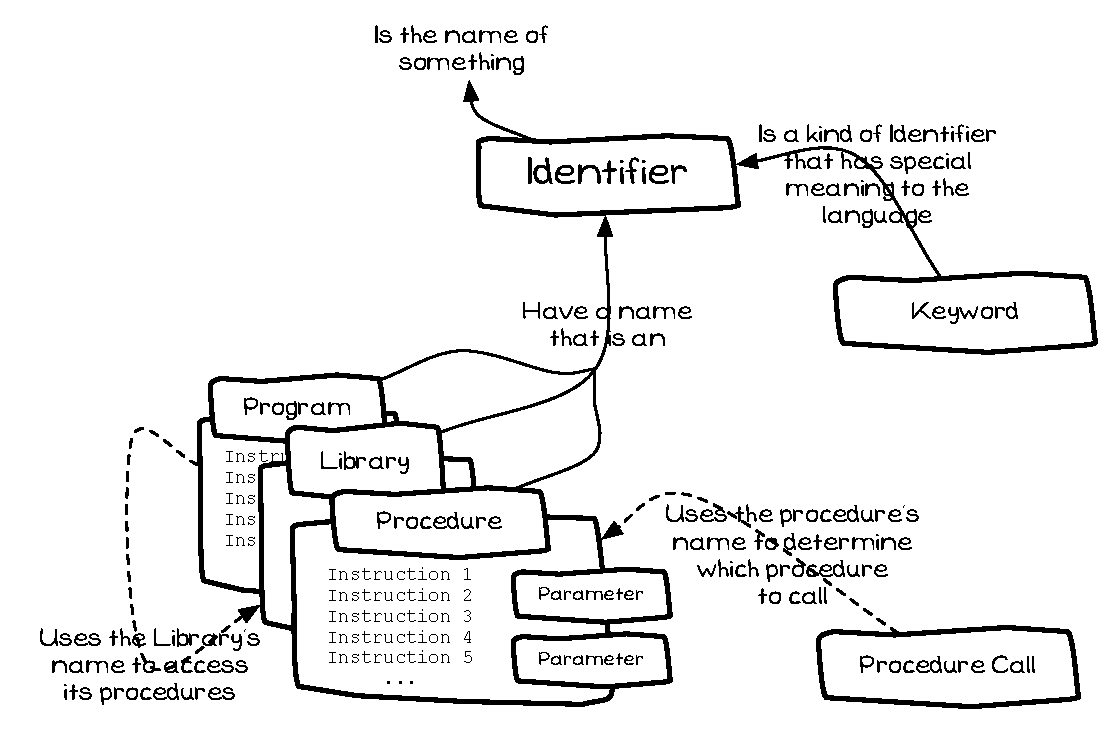
\includegraphics[width=\textwidth]{./topics/program-creation/diagrams/Identifier} 
   \caption[Identifier Concept Diagram]{An Identifier is the name of a programming artefact such as a Program, Library, or Procedure.}
   \label{fig:program-creation-identifier}
\end{figure}


\mynote{
\begin{itemize}
  \item Figure \ref{fig:program-creation-identifier} shows the concepts related to an Identifier.
  \item An Identifier is a \textbf{name} used to identify a programming artefact such as a \nameref{sub:program}, \nameref{sec:program-creation-library} or \nameref{sub:procedure}.
  \item The name you give your Program is an Identifier.
  \item You use Identifiers to indicate which Libraries you want to access in your Program.
  \item The \nameref{sub:procedure call} uses the Procedure's identifier to determine which procedure is called.
\end{itemize}
}

% section program (end)
\clearpage
\subsection{Library} % (fold)
\label{sec:program-creation-library}

A Library is a collection of reusable code artefacts. Each programming language has its own Library, and your programs can make use of the code available in this library.

\begin{figure}[h]
   \centering
   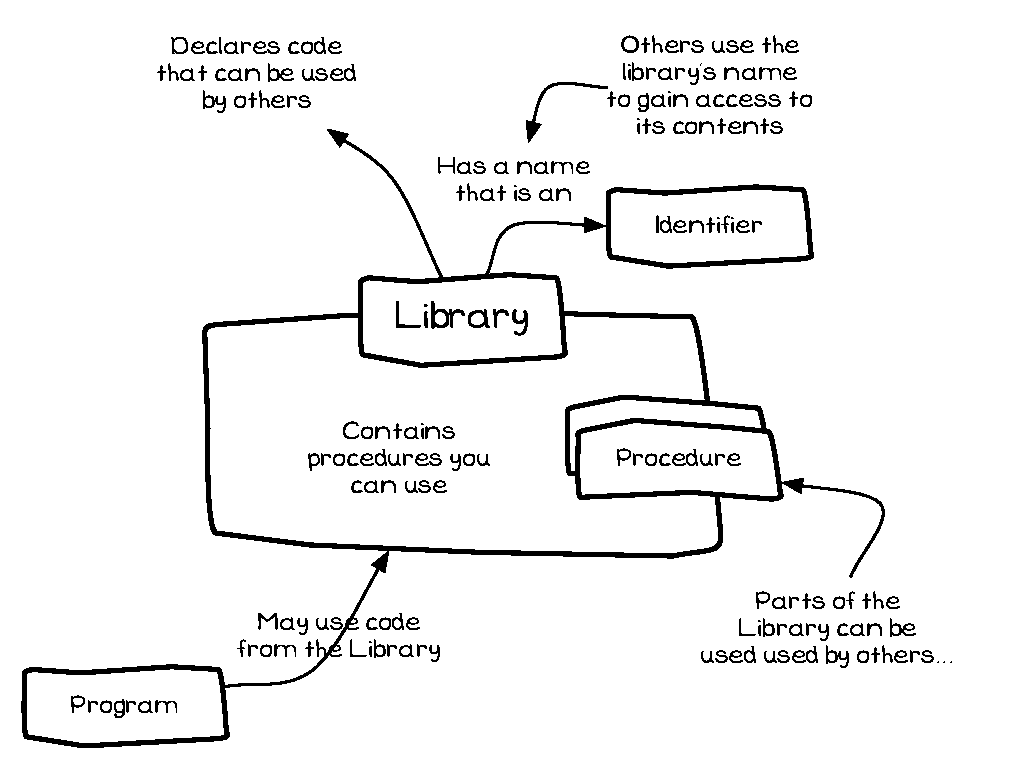
\includegraphics[width=\textwidth]{./topics/program-creation/diagrams/Library} 
   \caption[Library Concept Diagram]{A Library contains code that can be used by your Program}
   \label{fig:program-creation-library}
\end{figure}


\mynote{
\begin{itemize}
  \item Figure \ref{fig:program-creation-library} shows the concepts related to a Library.
  \item A Library is a collection of reusable code artefacts that you can use to perform certain tasks.
  \item The Library will contain \nameref{sub:procedure}s that perform a number of tasks.
  \item Each language has a standard library with code to perform many commonly performed tasks.
  \item Other libraries extend the capability of the languages further.
  \item SwinGame is a Library containing code to help you build games.
\end{itemize}
}

% section program (end)
\clearpage
\subsection{Comments} % (fold)
\label{sub:comments}

A program's source code contains instructions for the actions the computer must perform. However, this code is written and maintained by people. It is often useful to be able to place comments in the code to help someone reading that code understand how the code works or what it is trying to achieve. This text is not something that should be translated into machine code.

Programming languages include the ability to embed \emph{comments} that are ignored by the compiler when it compiles the code.

\bigskip

\mynote{
\begin{itemize}
  \item It is good practice to place a comment at the top of your code explaining what the program does.
  \item Comments should be included to help other people read your code. You will also find these comments useful when you return to your code after a long break.
  \item Make your comments meaningful, try to capture your intentions and ideas.
  \item Comments have no impact on the executable produced by the compiler.
\end{itemize}
}

% subsection comments (end)
\clearpage
\subsection{Procedure Declarations} % (fold)
\label{sub:proc_decl-procedure_declarations}

Procedures contain code that define the steps the computer performs when the procedure is called. In your Program you can define your own Procedures, allowing you to divide a program's tasks into separate Procedures.

\begin{figure}[h]
   \centering
   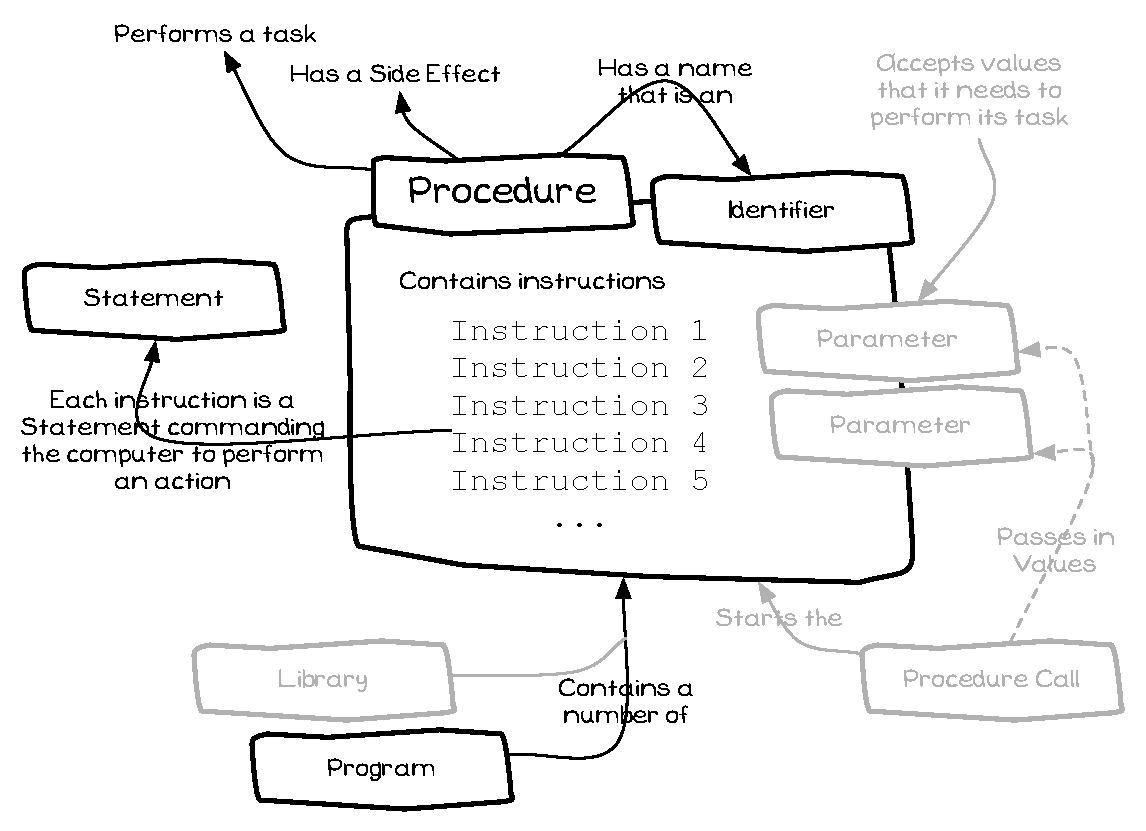
\includegraphics[width=\textwidth]{./topics/program-creation/diagrams/ProcedureDeclaration} 
   \caption{Procedure Declaration}
   \label{fig:procedure-decl-procedure-decl}
\end{figure}

\mynote{
\begin{itemize}
  \item A Procedure is an \textbf{artefact} that you can \emph{create} and \emph{use} in your code.
  \item Each Procedure contains code to perform a certain task. When you want the task performed you call the Procedure.
  \item Procedures should have a \textbf{side effect}\footnote{Output to the Terminal is an example of a Side Effect. After calling these procedures the text you wanted to appear was written to the Terminal. These Procedures changed the Terminal.}, meaning that it changes something when it is executed.
  \item The Procedure's declaration defines its \textbf{name}, and the \textbf{steps} it performs.
  \item Each instructions in the Procedure is a \nameref{sub:statement}.
  \item The Procedure's \nameref{sub:identifier}:
  \begin{itemize}
    \item Is the name used to call the Procedure.
    \item Should be a \textbf{verb} that \textbf{reflects the task} the Procedure performs.
  \end{itemize} 
  \item When the Procedure is called its instructions are executed.
  \item Each Procedure's instructions are isolated from the other code in your Program. When you are working on a Procedure you do not need to know about the internal workings of the other procedures.
\end{itemize}
}

% subsection procedure_declarations (end)

% section program_creation_concepts (end)

\clearpage
\subsection{Summary} % (fold)
\label{sub:program_creation_concepts_summary}

This section has introduced a number of programming artefacts, some programming terminology, and one kind of instruction. An overview of these concepts is shown in Figure \ref{fig:program-creation-summary}. The next section will look at how you can use these concepts to design some small programs.

\begin{figure}[h]
   \centering
   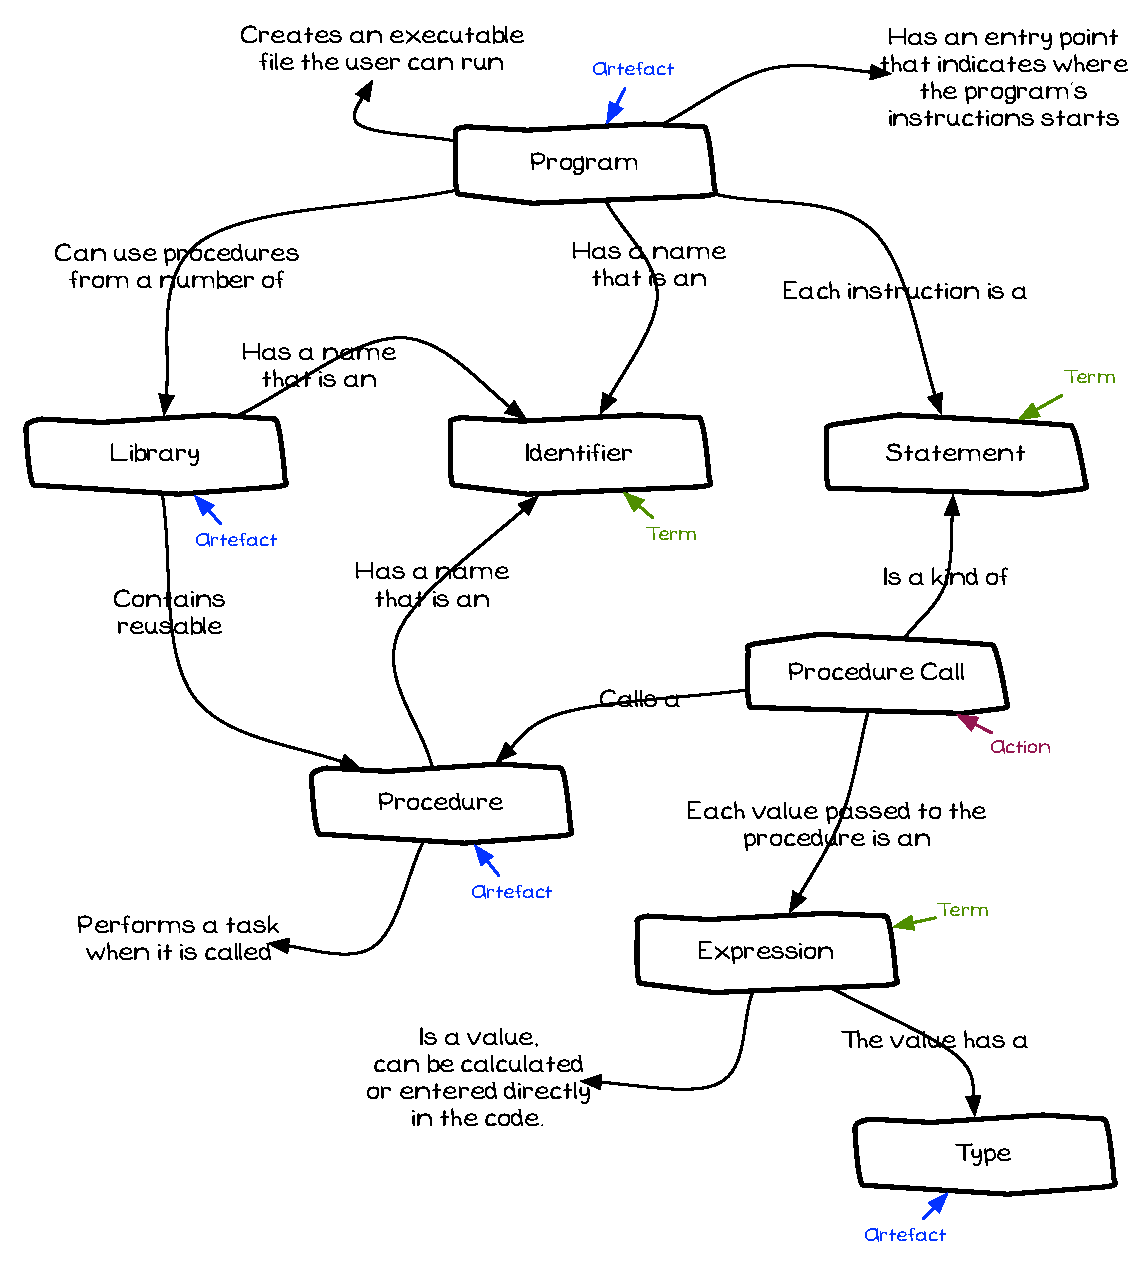
\includegraphics[width=\textwidth]{./topics/program-creation/diagrams/Summary} 
   \caption[Chapter Concepts]{Key Concepts introduced in this Chapter}
   \label{fig:program-creation-summary}
\end{figure}

\mynote{
\begin{itemize}
  \item \textbf{Artefacts} are things you can \emph{create} and \emph{use}.
  \item \textbf{Terms} are things you need to \emph{understand}.
  \item \textbf{Actions} are things you can \emph{command} the computer to perform.
\end{itemize}
}

% subsection summary (end)
